%!TEX root = ../../thesis.tex

\subsection{Tracks}
\label{sec:objects:tracks}

A track is a sequence of hits in the \ac{ID} indicative of a charged particle trajectory. 
To first approximation the trajectories are helical, owing to the pervading solenoidal 
magnetic field. However, multiple scattering and energy losses in the detector material 
and bremsstrahlung can cause significant deviations from this path. Track reconstruction 
is possible in the region $\mods{\eta} < 2.5$ (the extent of the \ac{ID}).

The inputs to the track reconstruction are threefold; pixel hits, \acs{SCT} space-points 
(each module comprises two layers of strips with a small stereo angle, enabling precise 
coordinate measurement), and \acs{TRT} drift circles. The \textit{inside-out} algorithm 
\cite{Tracking,ATLAS:ExpectPerf} uses a Kalman filter to seed tracks from hits in the 
three pixel layers and the first \acs{SCT} layer. The seeds are then extended and fitted 
through the \acs{SCT} and the \acs{TRT}, whilst resolving ambiguities and applying 
quality criteria. Finally, the \textit{outside-in} algorithm \cite{Tracking} considers 
unused track segments in the \acs{TRT}, and extrapolates them into the \acs{SCT} and 
pixel detector. This improves the tracking of secondary particles with a displaced vertex.



\subsection{Primary and secondary vertices}
\label{sec:objects:vertices}

A vertex is a location from which at least two outgoing tracks are reconstructed. 
\textit{Primary vertices} are associated with the interactions of incoming protons, 
whereas \textit{secondary vertices} are caused by particle decay or photon conversion
(\epluseminus pair production).

Primary vertex reconstruction has two steps: association of tracks to vertices 
(\textit{vertex finding}), and reconstruction of the vertex position itself 
(\textit{vertex fitting}). ATLAS employs an iterative \textit{finding-through-fitting} 
algorithm to simultaneously perform both steps \cite{PrimVertexFinding,AllVertexFinding}.
First, tracks originating from the interaction region 
(\unit{$\Delta z \approx 5.6$}{\centi\metre} and 
\unit{$\Delta r \approx 15$}{\micro\metre}) are identified and used to seed and fit a 
single vertex. Those tracks considered outliers are then used to seed a new vertex, and a 
second fit of the two vertices is performed. The algorithm iterates, increasing the 
number of vertices, until the result stabilises.

The total number of primary vertices \npv is used to assess the pile-up conditions of 
the bunch crossing. The primary vertex of the hard scatter is chosen to be that with the 
highest $\sum p_T^2$ of the constituent tracks, and is referred to as simply \textit{the} 
primary vertex. As an additional quality criterion, this vertex must have at least three 
associated tracks.

Secondary vertex reconstruction is highly constrained by the physics of the vertex 
\cite{AllVertexFinding}. This can be enforced by mass or angular constraints, or in the 
track selection. For example, photon conversions are found using oppositely charged 
collinear track pairs associated with electrons (using \acs{TRT} identification).
The \Pbottom-tagging of jets shall be described in \Section~\ref{sec:objects:bjets}.



\subsection{Electrons}
\label{sec:objects:electrons}

An electron will pass through the \ac{ID} before being absorbed by the \ac{ECal}. They 
are therefore reconstructed by matching a track with an energy cluster in the \ac{ECal}. 
Following reconstruction, the vast majority of electron objects are faked by hadrons, 
whilst many others are from photon conversions or electrons from heavy flavour decay (see 
\Figure~\ref{fig:electron_composition}). However, in the \HWWlvlv search, it is prompt 
electrons from the hard scatter that are of interest. Therefore identification and 
isolation criteria are applied to reject these backgrounds and select prompt electrons.

\begin{figure}
	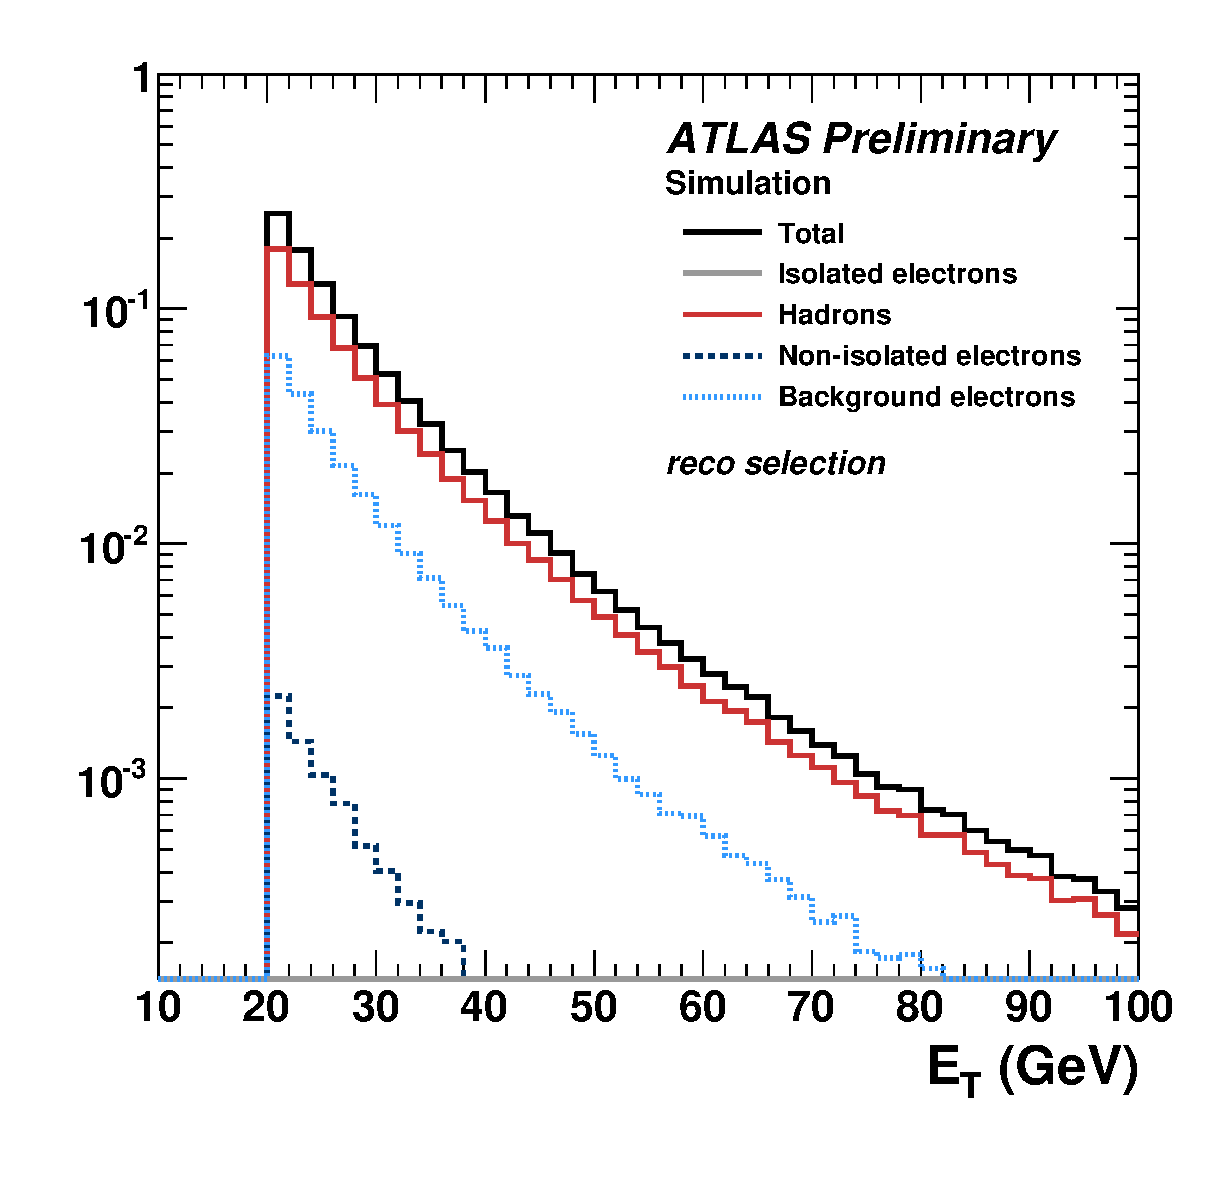
\includegraphics[width=\mediumfigwidth]{tex/selection/electron_composition}
	\caption{The composition of reconstructed electrons as a function of transverse 
	energy, simulated by a \pythia{6} sample of di-jet, heavy flavour, prompt photon, \PW 
	and \PZ processes \cite{ElectronPerf:Expect}. Non-isolated electrons are from heavy 
	flavour decay. Background electrons are from photon conversions. Isolated electrons 
	are prompt electrons from a \PW or \PZ boson, though appear below the y-axis range.}
	\label{fig:electron_composition}
\end{figure}

\begin{description}
\item[Reconstruction] \hfill \\
	Energy deposits in \ac{ECal} cells are clustered by a \textit{sliding window} 
	algorithm \cite{ElectronPerf:Expect}. First, the calorimeter is divided into radial 
	\textit{towers} of size $\Delta\eta \times \Delta\phi = 0.025 \times 0.025$, 
	corresponding to the cell size of the middle layer. Then a window of 3 \cross 5 towers
	in $\eta$-$\phi$ space scans the \ac{ECal} for local maxima with total transverse 
	energy greater than a threshold of \unit{2.5}{\GeV}. These are the seed clusters.

	For a seed cluster to be reconstructed as an electron, it must be matched to at least 
	one track. If a track (extrapolated to the middle \ac{ECal} layer) is within 
	$\Delta\eta < 0.05$ and $\Delta\phi < 0.1 (0.05)$ of the centre of the seed cluster, 
	they are considered matched. The asymmetric $\Delta\phi$ requirement allows for 
	increased bending due to bremsstrahlung. When multiple tracks are matched, that with 
	the smallest $\Delta R$ is chosen.

	Tracks associated to electron candidates are then refit using a Gaussian Sum Filter 
	(GSF) \cite{Electron:GSF}. This is because the default fit described in 
	\Section~\ref{sec:objects:tracks} uses a pion hypothesis to estimate material 
	effects, and does not account for the significant bremsstrahlung experienced by 
	electrons. The GSF is a non-linear fitter and can improve the accuracy of electron 
	tracking by accounting for this.


	final refit
	efficiency from Z tag-and-probe \cite{ElectronPerf:2010,ElectronPerf:2012}
	d0, z0 impact parameters
\item[Identification] \hfill \\
	very tight likelihood, medium++ cut-based
	efficiency from Z and J/Psi tag-and-probe \cite{ElectronPerf:2010,ElectronPerf:2012}
\item[Isolation] \hfill \\
	tracker and calo
\item[Four-momentum definition] \hfill \\
	energy from calo (EES EER calibration)
	direction from tracker
	pT > 10 GeV and cluster eta range (excl crack)
\end{description}



\subsection{Muons}
\label{sec:objects:muons}


\begin{description}
\item[Reconstruction] \hfill \\
	statistical combination of ID and MS tracks => STACO
	d0, z0 impact parameters
	track quality
\item[Isolation] \hfill \\
	tracker and calo
\end{description}


\subsection{Jets}
\label{sec:objects:jets}

topoclusters
energy scale calibration


\subsection{\Pbottom-jets}
\label{sec:objects:bjets}

MV1


\subsection{Missing transverse momentum}
\label{sec:objects:met}

hermetic design => incoming partons have very little transverse momentum => momentum conservation used to infer vector sum transverse momentum of non-interacting particles
True MET (neutrinos), Fake MET (mismeasurement, noise, etc)

\subsubsection{Track-based \met}

\subsubsection{Calorimeter-based \met}
